 \section{Aplicaciones}

\subsection{Resortes}


\subsection{Resortes}
\begin{figure}
	\centering
	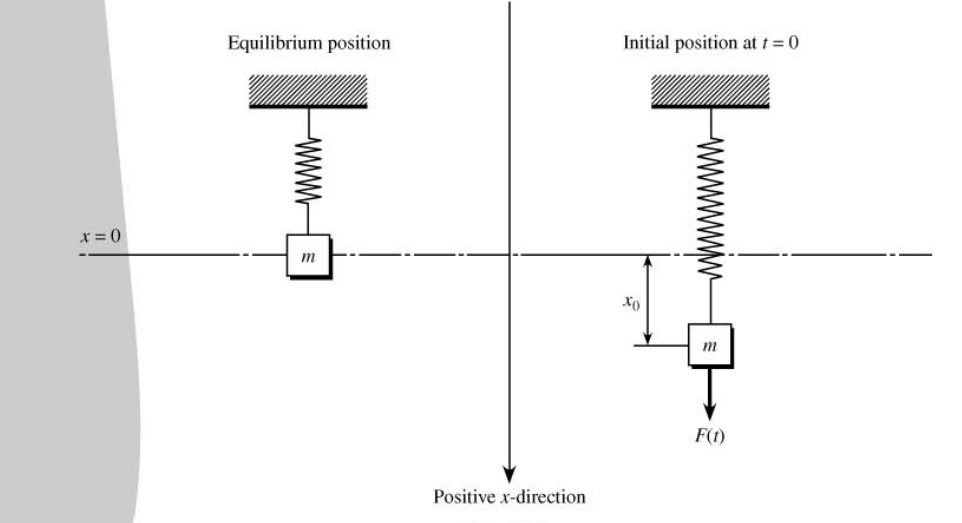
\includegraphics[height=5cm,keepaspectratio=true]{./edo/img030601.png}
	img030601.png: 0x0 pixel, 300dpi, 0.00x0.00 cm, bb=
	\label{fig:030601}
\end{figure}




\subsection{Ley de Hooke}
La fuerza restauradora $F$ de un resorte es igual y opuesta a las fuerzas aplicadas al mismo y proporcional a la extensi\'on (contracci\'on) $l$ del resorte de la fuerza aplicada, es decir, $F=-kl,$ donde $k$ indica la constante de proporcionalidad, generalmente llamada constante del resorte.



A partir de la segunda ley de Newton, tenemos que $$m\ddot{x}=-kx-a\dot{x}+F(t),$$ o de manera equivalente
\[
	\label{bron:14.1}
	\ddot{x}+\dfrac{a}{m}\dot{x}+\dfrac{k}{m}x=\dfrac{F(t)}{m},
\]
donde $a,k$ son constantes positivas de proporcionalida; $F(t)$ es una fuerza externa; y sujeta a condiciones iniciales
\[
	\label{bron:14.2}
	x(0)=x_{0}, \dot{x}(0)=v_{0}.
\]




\begin{resuelto}
	\label{bron:exmp:14.2}
	Una masa de $2kg$ se suspende de un resorte con una constante conocida de $10N/m,$ y se le permite llegar a una posici\'on de reposo. Luego se le pone en movimiento dándole una velocidad inicial de $150cm/seg.$ Encuentre una expresi\'on para el movimiento de la masa, suponiendo que no hay resistencia del aire.
\end{resuelto}




\begin{resuelto}
	Encuentre la frecuencia circular; la frecuencia natural y el periodo el oscilador arm\'onico simple del problema \ref{bron:exmp:14.2}.
\end{resuelto}



\subsection{Círcuitos eléctricos}


\begin{figure}
	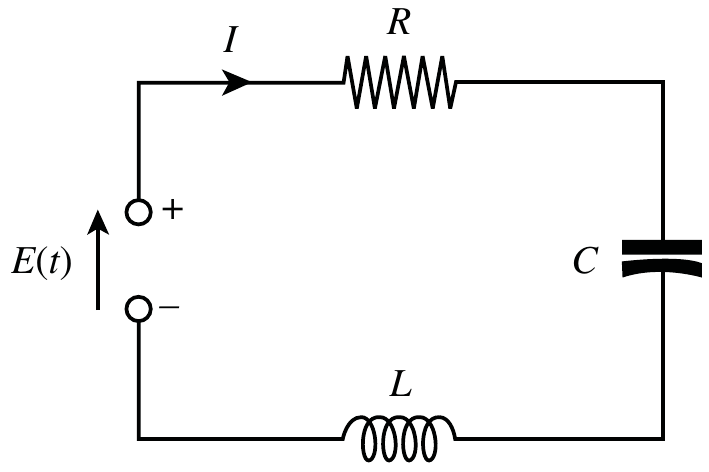
\includegraphics[height=7cm,keepaspectratio=true]{./edo/circuitos_electricos.png}
	\label{fig:circuitos}
\end{figure}



{}
\begin{itemize}
	\item Cantidad de corriente $I$ (en amperios)
	\item Resistencia $R$ (en ohmios)
	\item Inductor $L$ (en henrios)
	\item Fuerza electromotriz (abreviado fem)$E$ (en voltios)
	\item Capacidad $C$ (en faradios)
\end{itemize}


{La ley del bucle de Kirchhoff}
La suma algebraica de las caídas de voltaje en un circuito eléctrico cerrado simple es cero.


{}
\begin{align*}
	RI + L\dfrac{dI}{dt}+\dfrac{1}{C}q-E(t)=0
\end{align*}


{}
\begin{align*}
	I&=\dfrac{dq}{dt}\\
	\dfrac{dI}{dt}&=\dfrac{d^{2}q}{dt^{2}}
\end{align*}



{}
\begin{align*}
	\dfrac{d^{2}q}{dt^{2}}
	+\dfrac{R}{L}\dfrac{dq}{dt}
	+\dfrac{1}{LC}q =
	\dfrac{1}{L}E(t)
\end{align*}


{}
\begin{align*}
	q(0) &= q_{0}\\
	I(0) &= \evat{\dfrac{dq}{dt}}{t=0}=I_{0}
\end{align*}


{}
\begin{resuelto}
	Un circuito RCL conectado en serie tiene $R = 180$ ohmios, $C = 1/280$ faradio, $L = 20$ henries, y una aplicada
	voltaje $E(t) = 10 \sen t$.


	Suponiendo que no hay carga inicial en el capacitor, sino una corriente inicial de 1 amperio en
	$t = 0$ cuando se aplica la tensión por primera vez, encuentre la carga subsiguiente en el capacitor.
\end{resuelto}



